% Use class option [extendedabs] to prepare the 1-page extended abstract.
\documentclass[extendedabs]{bmvc2k}
\usepackage[colorlinks = true,
            linkcolor = blue,
            urlcolor  = blue,
            citecolor = blue,
            anchorcolor = blue]{hyperref}
\usepackage{kotex} % 한국어 사용 가능

% Document starts here
\begin{document}
\title{Convolutional Neural Networks : LeNet, VGG, ResNet}
\addauthor{
Lee Gwan Hui$^1$, \today}{}{1}
\addinstitution{
$^1$2017142136, Department of Electrical and Electronic Engineering, Yonsei University.}
\maketitle
\let\thefootnote\relax\footnote{This is an extended abstract. The full paper is available at the \href{https://github.com/LeeGwanHui/TIL/tree/main/deeplearning_ham}{github}. }
\vspace{-0.2in}

\section{abstract}

 1998년 LeNet-5\cite{lecun1998gradient}가 발표되었지만 당시의 기술적 한계인 연산속도 때문에 CNN은 크게 주목을 받지 못했다.
 2010년에서 2017년까지 진행한 ILSVRC에서 2012년 AlexNet\cite{krizhevsky2012imagenet}이 연산속도의 발전으로 CNN based 기반 model로 우승을 차지하고
 이미지 처리 분야에서 전통적인 알고리즘으로 CNN 기반 모델의 성능을 뛰어넘지 못함으로써 CNN이 장족의 발전이 진행되었다.
 이 보고서에는 ILSVRC 14의 준우승 VGG model\cite{simonyan2014very} 과 ILSVRC 15 우승 ResNet\cite{he2016deep}을 구현한 논문을 읽고 요약정리를 진행할 것이다.

 \section{Very Deep Convolutional Networks for Large-Scale Image Recognition}
 이 논문은 3x3 conv filter을 통해 layer의 depth를 늘려서 large-scale image recognition에서 높은 정확도을 얻은 과정을 설명하고 있다.
 이 논문에서 구성한 구조를 가지고 ImageNet Challenge 2014에 참여하였고 GoogleNet 다음으로 준우승을 차지하였다.

 \subsection{VGG의 구성}
 conv.net을 사용하여 image recognition에 많은 발전이 일어났다. 이를 가능케 해준 것은 GPU의 발전과 ILSVRC의 덕분이라고 할 수 있다.
 이 논문을 전체적으로 요약하자면 ConvNet architecture에서 depth의 중요성을 나타낸 것으로 이를 가능토록하기 위해 3x3 convolution filter을 사용하였다.
 VGG의 architecture을 살펴보자.
 \newline Input size : 224 x 224 RGB image.
 \newline filter size : 3x3 filter, 1x1 filter(a linear transformation of the input channels의 역할)
 \newline convolution stride : 1 pixel
 \newline padding size : 1 pixel for 3x3 conv.layer (because the spatial resolution is preserved after convolution)
 \newline pooling : Max-pooling 사용 (2x2 pixel window, with stride 2)
 \newline rectification : ReLU 를 사용해서 non-linearity 성질을 삽입시킴.
 \newline the configuration of the fully connected layers is followed by three FC layers.
 \newline the final layer is the soft-max layer.
 \newline 위의 구조를 바탕으로 아래 그림은 VGG16를 도식화한 그림이다.
 \newline  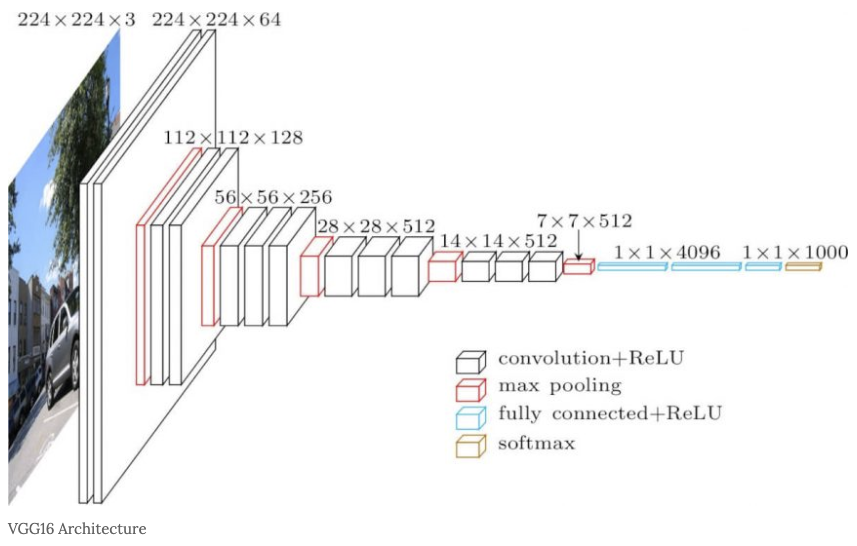
\includegraphics[width=6cm, height=4cm]{images/01_VGG.png}
 \newline  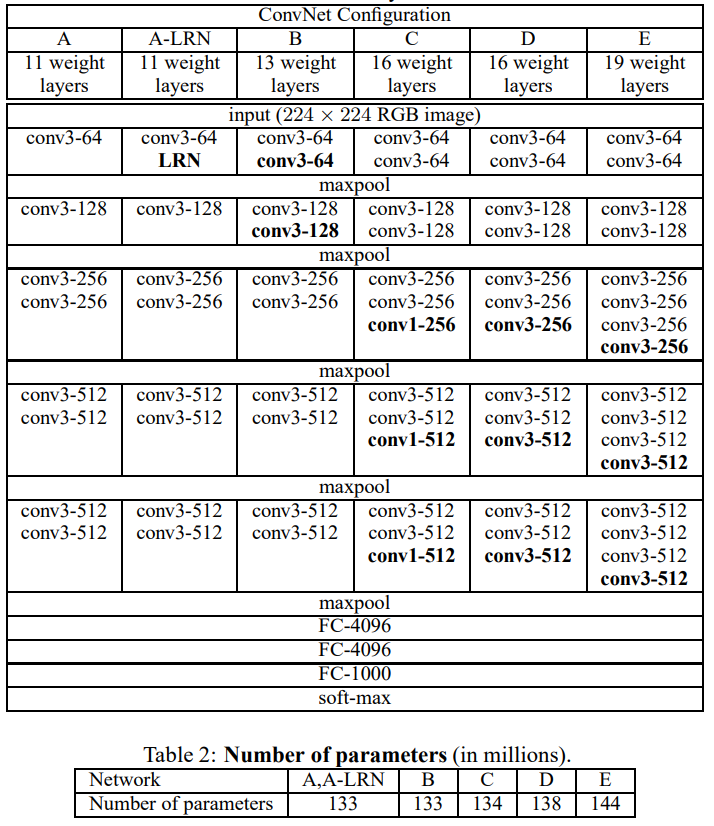
\includegraphics[width=\linewidth]{images/02_VGG.png}
 \newline  \textbf{discussion} 여기서 논할 것은 VGG net이 어떻게 layer depth을 늘렸는가이다. 
 layer depth을 늘리는 만큼 기존에는 parameter수가 같이 증가했기 때문에 일정 이상 늘리는 것에 한계가 있었다.
 이를 해결하기 위해 3x3 conv filter을 이용해서 layer을 구성하였고 이를 통해 depth을 늘릴 수 있었다.
 이 뜻을 이해하기 위해서는 receptive field라는 개념을 알 필요가 있다. receptive field란 convolutional filter에서 
 파생된 개념으로 이미지를 예로 들면 filter을 통과한 값이 이미지의 어느 영역을 보고 값을 도출했는지를 나타내는 말이다. 
 개념에서 알 수 있듯이 receptive field가 크면 더 넓은 범위를 보고 물체가 무엇인지 파악하기 때문에 이미지의 정확도를 
 일부 높일 수 있는 hyperparameter이다. 너무 receptive field가 적은 예를 들면 개 사진에서 피부만을 보고 개인지 
 판단해야 하는 경우가 생길 수가 있다. 그러나 receptive field가 너무 커버리면 세부 특징들을 잡아내지 못함으로써 정확도가 낮아진다.
 보통 이전까지의 연구에서 5x5 혹은 7x7을 사용한 것으로 보아 이 크기가 특징을 잘 잡아낼 수 있을 것으로 추측할 수 있다.
 3x3 convolutional filter을 사용하면서도 receptive field을 늘리기 위해서는 여러번 통과 시키면 된다는 것을 깨달은 본 연구자들이 이를 적용하였다.
 이를 그림으로 표현하면 아래와 같다.
 \newline  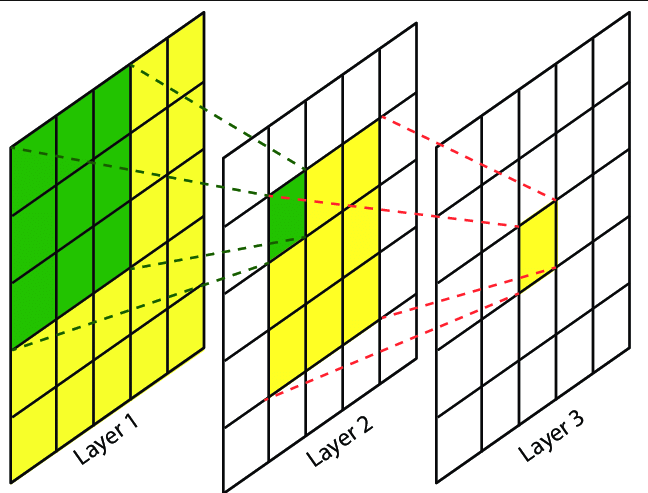
\includegraphics[width=5cm, height=3cm]{images/03_VGG.png}
 \newline 3x3 filter을 두번 통과시키면 receptive field(노란색) 5x5가 됨을 볼 수 있다. 그럼 같은 receptive field을 위해 왜 7x7 대신 3x3 filter 3개를 사용하는가에 대한
 문제를 살펴보자. 우선 parameter의 수가 줄어든다. $3(3x3xC^2)$ 와 $7x7xC^2$ 을 비교해보면 앞에 값이 27$C^2$으로 더 낮은 parameter을 사용한 것을 알 수 있다. 또한 
 추가로 layer을 통과할 때 non-linearity 추가를 위해 ReLU을 통과시키는데 이 행위가 여러번 반복되면서 non- linear한 문제를 더 잘 풀 수 있게 도와 준다.(만약
 activation function을 통과시켜주지 않으면 ABx가 되어 사실상은 Cx와 같다. 이 말은 A layer 통과 후 B layer 통과한 것과 사실이와 같은 C layer 하나만 통과한 것과 마찬가지이다.)

\subsection{Train and Testing procedures}
 논문에서 training과 testing의 마지막 FC 구조를 다르게 설정하였다. 최근 연구는 같게 구현하는 경우가 많기 때문에 중요한 내용은 아니다. 그러므로 여기서는 training과 testing의
차이보다는 어떤 식으로 training set을 구성했는지를 중점으로 볼 것이다.
\newline  \textbf{Training}
 먼저 training에서는 Cross entropy loss를 사용하고 mini-batch gradient descent를 이용하였다. batch size는 256로 설정하고 (요즘 연구에는 32,64를 많이 사용한다고 한다.)
 momentum=0.9, L2 regularization(Least squares error(LSE)), Dropout=0.5, learning rate 초기 $10^{-2}$에서 10배씩 감소 등의 hyperparameter을 설정하고 74 epochs을 돌렸다.
 이 논문에서 자랑하는 것이 더 많은 parameter, depth을 사용했음에도 불구하고 수렴은 더 빨랐다는 것인데 이 이유로 (a) implicit regularization imposed by greater depth and smaller conv. filter sizes 
 (b) pre-initialization of certain layers 두가지를 들었다. 그리고 training scale S에 대해 두가지 방법을 사용했는데 한가지는 S를 고정하고 traning 시킨 것이고 두번째 방법으로는
 [$S_{min}, S_{max}$]범위에서 random하게 rescale시켜 진행하였다.
\newline  \textbf{Testing}
 Testing에서는 S와 같아도 되고 달라도 되는 Q를 사용하였고 FC layer도 trick를 이용하여 FC convolutional layer로 변경해주었다.
\newline  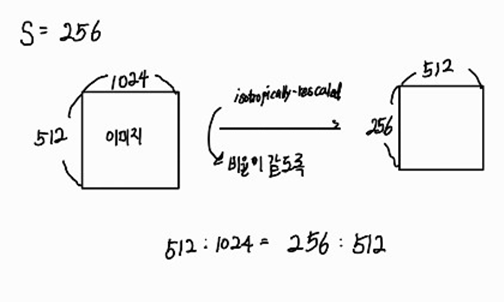
\includegraphics[width=5cm, height=3cm]{images/04_VGG.png}

\subsection{Conclusion}
 normalization, ensemble을 적용하여 ILSVRC 14 최종 2등을 차지 하였다. 이 논문에서 가장 중요한 것은 3x3 filter가 매우 합리적이고 성능이 좋다는 것과 layer의 depth을 높일 수록
 더 높은 정확도를 가진다는 것이다. 이 이유에 대해서는 나중에 low level feature과 high level feature이 사람이 보기에도 더 의미 있는 feature을 추출해 낸다는 것이 밝혀졌다. 
 \newline  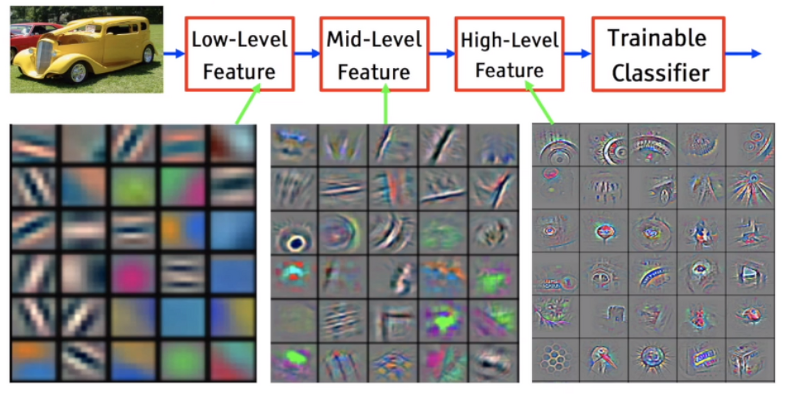
\includegraphics[width=\linewidth]{images/08_residual.PNG}

\section{Deep Residual Learning for Image Recognition}
논문의 흐름을 보면 합리적이다. VGG 논문에서 layer의 depth가 높을수록 정확도가 높다는 것을 밝혔다. 그럼 layer을 더 쌓기만 하면 정확도는 더 오를까라는 자연스러운 질문으로
layer을 56개까지 쌓았고 그 결과 20 layer보다 성능이 떨어진 degradation problem을 발견하였다. 이는 train, test error 모두 20 layer에 비교해서 높아 overfitting문제는 아니다. 이 논문은
이 문제를 해결하고 layer의 depth을 높여 정확도를 높이는 것을 목적으로 진행되었다. 여기서는 residual function을 사용하여 degradation problem을 해결하고자 하였다.
 \newline  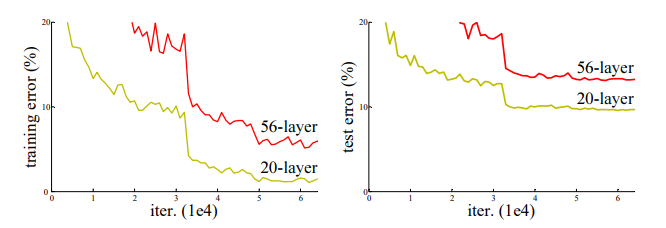
\includegraphics[width=\linewidth]{images/09_residual.PNG}
\subsection{ReNet 구성}
degradation을 원인을 multiple nonlinear layer 때문이라고 규정하고 layer을 재구조화하였다. 이 때 추가된 layer은 identity mapping이고 나머지 layer은 learned shallower model로 구성하였다. 
구조를 살펴보면 아래와 같다. 설명하자면 여태 학습한 방법은 H(x)함수로 true 값에 가까워지는 것이었다. 그러나 ResNet에서는 H(x)-x=F(s)를 학습하기 때문에 업데이트하는 weight가 차이가 있다.
이를 진행한 가설은 H(x)보다 F(X)를 optimize 시키는 것이 더 쉽다는 가정이다. 이 이유로 만약 입력과 똑같은 출력을 원한다면 H(x)의 경우 identity matrix가 되어야 하지만
F(x)의 경우에는 zero matrix기만 하면 되기 때문이라는 예시를 들었다. F(X)을 식으로 나타내면 $F=W_2\sigma(W_1x)$ 같이 나타낼 수 있다. 여기서 $\sigma$는 ReLU을 의미한다.   
\newline  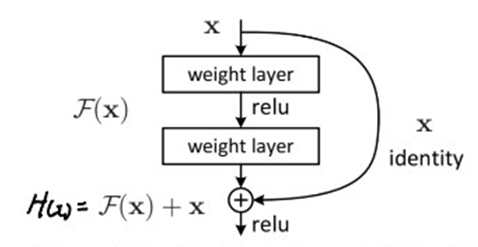
\includegraphics[width=6cm, height=4cm]{images/10_residual.PNG}
\newline 위의 그림에 나타내고 있는 단위를 residual block이라고 부르면 residual block 안에는 3x3 conv layer이 두개로 구성되어 있고 주기적으로 feature map을 2배로 
special dimension은 1/2배로 조정한다. 이를 모델 전체적으로 나타내면 아래와 같다. 
\newline  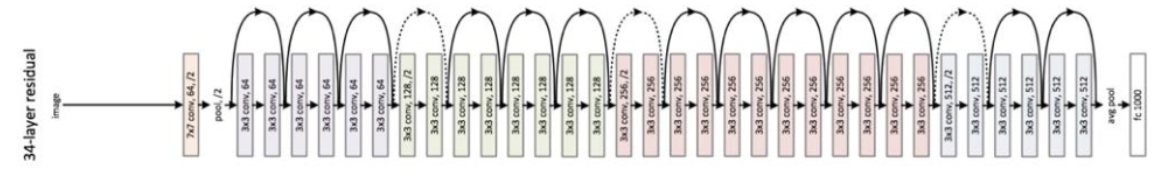
\includegraphics[width=\linewidth]{images/11_residual.PNG}
\newline 기본 구성은 VGG net을 참고하였고 여기서 추가적으로 skip connection을 추가하였다. downsampling은 stride가 2인 conv layer을 통과로 구현하였다.
그리고 network의 마지막에는 global average pooling layer과 FC layer과 softmax가 구현되어 있다.

\subsection{Experiments}
실행은 VGG net과 거의 비슷하고 차이를 언급하자면 ResNet 실험에서는 dropout을 사용하지 않았다. 실험 결과 plain Network의 경우
degradation problem이 발생하였고 forward, backward signals vanish 때문은 아니라고 밝혔다. 그리고 이 이유를 exponentially low convergence rates 때문이라고 추측했다.
이를 해결하기 위해 residual Network를 사용한 결과 수렴속도는 더 빠르고 error도 감소하였다. 여기까지 실험한 것이 18,34 layer ResNet이다. 
layer의 depth을 더 늘리기 위해서는 bottleneck architecture을 이용하여 complexity를 줄일 필요가 있다. 처음 들어오는
1x1 conv 에서 3x3 conv에서 handling하는 계산량을 줄이고 다시 1x1 conv로 원래대로 회복하는 형태로 설계하였다.
\newline  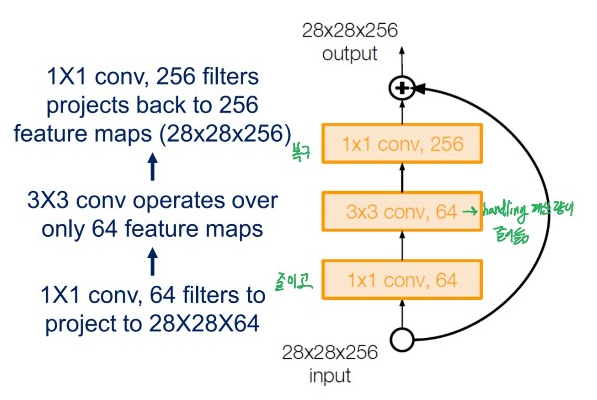
\includegraphics[width=\linewidth]{images/12_residual.PNG}
\newline bottleneck, residual을 이용한 152-layer ResNet은 VGG-16,19보다 더 낮은 complexity를 가지고 있다. 실험결과 degradation 문제를 해결만 해주면 
layer의 depth가 증가할수록 정확도는 높아진다는 것을 증명하였다.

\subsection{Conclusion}
이 논문은 Residual connection을 이용해 layer을 더 깊이 쌓을 수 있는 구조적 형태를 제시함으로써 ILSVRC 15 우승의 결과를 만들어 냈다. 3x3 convolution을 반복적으로 쌓은 구조에서
residual layer을 추가함으로써 매우 간단하여 오늘날 까지 가장 널리 쓰이는 model이 되었다.

\section{전체적인 요약}
 아래 그림은 중요 model의 성능을 비교 분석한 것이다.\cite{canziani2016analysis} 여기서 위에서 리뷰한 2개의 model(VGG, ResNet)을 살펴보면 ResNet의 경우에는 정확도와 operation 모두 
 VGG를 능가한 것을 볼 수 있다. 물론 시간이 지나면서 더 좋은 모델(Inception-v4)가 나왔지만 그럼에도 위에서 언급했듯이 ResNet이 주로 사용되고 있다.
 \newline  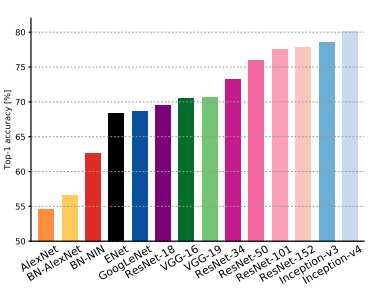
\includegraphics[width=5cm, height=3cm]{images/13_sumary.PNG} 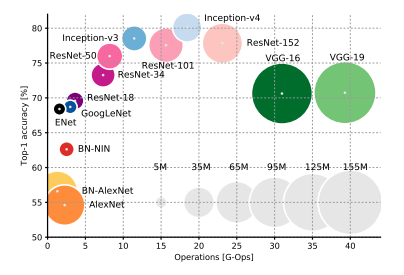
\includegraphics[width=5cm, height=3cm]{images/14_sumary.PNG}

\newpage
\bibliography{egbib}

\end{document}
